% Homework 1 -- Lecture 1: data, descriptive statistics and probability. Paper only.
% The data come from hw01_data.tex, written by hw01_numbers.py (every number computed and unit-tested).
% generated by hw01_numbers.py -- do not edit
\newcommand{\hwRents}{510,\ 450,\ 1{,}450,\ 420,\ 560,\ 470,\ 450,\ 530,\ 480}
\newcommand{\hwDelA}{23,\ 27,\ 25,\ 24,\ 26}
\newcommand{\hwDelB}{15,\ 35,\ 20,\ 30,\ 25}
\newcommand{\hwScores}{63,\ 41,\ 75,\ 58,\ 98,\ 52,\ 70,\ 61,\ 55,\ 72,\ 66}
\newcommand{\hwErrData}{2,\ 4,\ 6,\ 8}
\newcommand{\hwStaff}{49}
\newcommand{\hwStaffPay}{1{,}200}
\newcommand{\hwOwnerPay}{380{,}000}
\newcommand{\hwBdayA}{5}
\newcommand{\hwBdayB}{30}
\newcommand{\hwNewsClaim}{9{,}000}
\newcommand{\hwWrongVar}{mean $5$, so $s^2 = \frac{(2-5)^2 + (4-5)^2 + (6-5)^2 + (8-5)^2}{4} = \frac{20}{4} = 5$}


\section*{Homework 1: Data, Descriptive Statistics and Probability}
\noindent\textbf{Lecture 1.} Work on paper, by hand: a pen, a ruler and a basic calculator only. Show every step,
because the exam is on paper too and a correct method earns most of the marks. Use the lecture's conventions: the
sample variance divides by $n-1$; quartiles are the medians of the lower and upper halves (leave the median out when
$n$ is odd); an outlier lies beyond $Q_1 - 1.5\,\mathrm{IQR}$ or $Q_3 + 1.5\,\mathrm{IQR}$.

\subsection*{Task 1. What kind of data? \hfill (6 points)}
For each variable say whether it is \emph{nominal}, \emph{ordinal}, \emph{discrete} or \emph{continuous}, and whether
its mean would mean anything.
\begin{enumerate}[label=(\alph*), itemsep=0pt]
  \item a student's postcode
  \item the number of siblings a student has
  \item the time a runner needs for 5\,km
  \item blood type (A, B, AB, O)
  \item a hotel rating: poor / fair / good / excellent
  \item the number of emails a person receives in a day
  \item the temperature at noon, in $^\circ$C
  \item T-shirt size: S, M, L, XL
\end{enumerate}
Then explain in one sentence why a variable written with digits (like (a)) can still be categorical.

\subsection*{Task 2. Where is the centre? \hfill (8 points)}
The monthly rents (\$) of nine flats in one street are
\[ \hwRents. \]
\begin{enumerate}[label=(\alph*)]
  \item Write the data as $x_1, \dots, x_9$ in the order given, and compute $\sum_{i=1}^{9} x_i$.
  \item Compute the mean, the median and the mode.
  \item How many of the nine flats are cheaper than the mean? Which of the three numbers describes a \emph{typical}
        flat in this street, and why?
  \item The most expensive flat is removed. Compute the new mean and median. Which one moved more, and why?
  \item The mean is above the median. What does that tell you about the shape of the data?
\end{enumerate}

\subsection*{Task 3. Same mean, different spread \hfill (8 points)}
Two delivery services brought five orders each. Delivery times in minutes:
\[ \text{Service A: } \hwDelA \qquad\qquad \text{Service B: } \hwDelB \]
\begin{enumerate}[label=(\alph*)]
  \item Show that both services have the same mean.
  \item For each service make a table with columns $x_i$, $x_i - \bar{x}$ and $(x_i - \bar{x})^2$, and compute $s^2$ and
        $s$.
  \item Add up the column $x_i - \bar{x}$. What do you get, and why does that force us to square the deviations?
  \item You need a delivery for a meeting that starts in 30 minutes. Which service do you choose, and which number
        from (b) supports your choice?
\end{enumerate}

\subsection*{Task 4. Five numbers and a box plot \hfill (10 points)}
The exam scores of eleven students are
\[ \hwScores. \]
\begin{enumerate}[label=(\alph*)]
  \item Sort the scores and find the five-number summary: minimum, $Q_1$, median, $Q_3$, maximum.
  \item Compute the IQR and both fences. Which score, if any, is an outlier?
  \item Draw the box plot on the axis below: the box from $Q_1$ to $Q_3$, a line at the median, whiskers to the most
        extreme scores that are \emph{not} outliers, and each outlier as a separate dot.
  \item The top score is replaced by a much larger number by mistake. Which of the five numbers change, and does the
        IQR change? Explain.
\end{enumerate}
\begin{center}
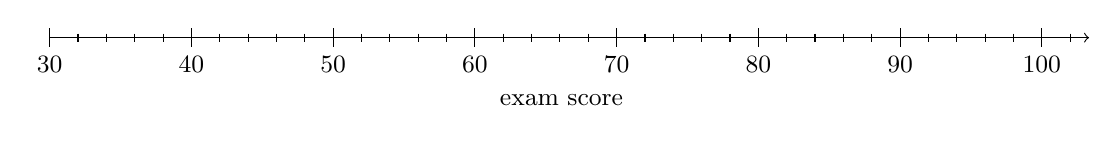
\begin{tikzpicture}
  \draw[->] (0,0) -- (13.2,0);
  \foreach \v in {30,40,...,100} {
    \pgfmathsetmacro{\x}{(\v-30)*0.18}
    \draw (\x,0.12) -- (\x,-0.12) node[below] {\small\v};
  }
  \foreach \v in {30,32,...,102} { \pgfmathsetmacro{\x}{(\v-30)*0.18} \draw (\x,0.05) -- (\x,-0.05); }
  \node[below] at (6.5,-0.6) {\small exam score};
\end{tikzpicture}
\end{center}

\subsection*{Task 5. Your own data: sixty rolls of a die \hfill (8 points)}
Roll an ordinary die 60 times and record each result in the table with tally marks.
\begin{center}
\renewcommand{\arraystretch}{1.6}
\begin{tabular}{|c|p{5.5cm}|c|c|}
\hline
Face & Tally & Frequency & Relative frequency \\ \hline
1 & & & \\ \hline 2 & & & \\ \hline 3 & & & \\ \hline
4 & & & \\ \hline 5 & & & \\ \hline 6 & & & \\ \hline
Total & & 60 & 1 \\ \hline
\end{tabular}
\end{center}
\begin{enumerate}[label=(\alph*)]
  \item Draw a bar chart of the frequencies. Should the bars touch, as in a histogram? Explain.
  \item Write down the sample space $\Omega$ and the event $A=$ ``an even number''. Give the classical $P(A)$ and the
        empirical $P(A)$ from your rolls.
  \item How many times would you \emph{expect} each face in 60 fair rolls? Which face is furthest from that, and do
        you think your die is unfair? (You will learn to test this properly in Lecture 10; here, just argue.)
\end{enumerate}

\subsection*{Task 6. Probability rules \hfill (12 points)}
\begin{enumerate}[label=(\alph*)]
  \item One card is drawn from a standard deck of 52. Find $P(\text{red} \cup \text{queen})$ with the addition rule.
        Which cards would you count twice without the correction?
  \item Two dice are rolled. List the sample space as a $6 \times 6$ grid and find $P(\text{sum} = 7)$ and
        $P(\text{sum} \ge 10)$.
  \item Find $P(\text{at least one six})$ for two dice twice: by counting cells in your grid, and with the complement
        rule. Then use the complement rule for four dice.
  \item One die, $A = \{2,4,6\}$. For each of $B=\{1,2,3\}$, $C=\{1,2,3,4\}$ and $D=\{1,3,5\}$, decide whether it is
        independent of $A$ and whether it is mutually exclusive with $A$. Show the numbers you compare.
  \item Use the complement rule to find the probability that at least two people share a birthday in a group of
        \hwBdayA{} and in a class of \hwBdayB{} (365 equally likely days, no leap years). Write the product out for the
        group of \hwBdayA.
\end{enumerate}

\subsection*{Task 7. Find the errors \hfill (6 points)}
A classmate handed in the solution below. Each part contains one error. Find it, explain it, and correct the answer.
\begin{enumerate}[label=(\alph*)]
  \item ``The sample $\hwErrData$ has \hwWrongVar.''
  \item ``One card from 52: $P(\heartsuit \cup \mathrm{K}) = P(\heartsuit) + P(\mathrm{K}) =
        \frac{13}{52} + \frac{4}{52} = \frac{17}{52}$.''
  \item ``On one die, `even' and `odd' can never happen together, so they are independent.''
\end{enumerate}

\subsection*{Task 8. Explain it in words \hfill (4 points)}
A small company has \hwStaff{} employees who each earn \$\hwStaffPay{} a month, and an owner who pays herself
\$\hwOwnerPay{} a month. A newspaper writes: ``The average monthly pay at this company is almost \$\hwNewsClaim.''
Compute the mean and the median monthly pay of all \hwStaff{} + 1 people. Is the newspaper wrong? Which number would
you report to someone who wants to work there, and why? (Three or four sentences.)

\subsection*{Optional challenge \hfill (+4 points)}
\begin{enumerate}[label=(\alph*)]
  \item Show that for any sample $\sum_{i=1}^{n}(x_i - \bar{x}) = 0$.
  \item Show that $\sum_{i=1}^{n}(x_i - \bar{x})^2 = \sum_{i=1}^{n} x_i^2 - n\bar{x}^2$, and use it to check your $s^2$ for
        service B in Task 3.
\end{enumerate}

\medskip
\noindent\textbf{Total: 62 points} (+4 optional). Hand in your handwritten pages, with your name on each page.
